\documentclass[11pt]{article}
\usepackage[margin=1in]{geometry}
\usepackage{volfit_preamble}
\graphicspath{{figures/}}

\title{\textbf{Messages, Not Smoothness}\\[2pt]
\large The precision-message graph: every edge a contract, every contract a
Gaussian factor, and the global solve as the accountant\\[2pt]
\normalsize Vol-Fitter Technical Notes, No.~14}
\author{Vol-Fitter}
\date{\today}

% Note-local notation.
\newcommand{\Qmsg}{Q_{\mathrm{msg}}}
\newcommand{\Ldir}{L_{\mathrm{dir}}}
\newcommand{\Qdel}{Q_{\Delta}}

\begin{document}
\maketitle

% Generated numbers.  graph_messages_tables.tex carries everything unique to
% this edition (gen_graph_messages.py); the Phase-0 empirical numbers are
% read from the stored design-study artifact, never re-run.
% Auto-generated by gen_graph_messages.py — do not edit.
\newcommand{\gmthreem}{2.00}
\newcommand{\gmoney}{0.50}
\newcommand{\gmdeadhalf}{0.40}
\newcommand{\gmpairflat}{1.00}
\newcommand{\gmrepeatvar}{1.67}
\newcommand{\gmnaivevar}{1.20}
\newcommand{\gmrepeatratio}{1.39}
\newcommand{\gmcompetecancel}{0.00}
\newcommand{\gmcompeteout}{-0.50}
\newcommand{\gmcompetebeta}{0.75}
\newcommand{\gmrhoindex}{0.391}
\newcommand{\gmrhopeer}{0.762}
\newcommand{\gmtwosource}{0.561}
\newcommand{\gmuplift}{43}
\newcommand{\gmupliftbar}{15}
\newcommand{\gmphasen}{1007}
\newcommand{\gmpredtwo}{0.563}
\newcommand{\gmpredgap}{0.3}
\newcommand{\gmhopmean}{1.000}
\newcommand{\gmhopsdgap}{0.0000}
\newcommand{\gmpzero}{1690}
\newcommand{\gmepst}{0.97}
\newcommand{\gmtauonem}{2.7}
\newcommand{\gmcalpairs}{11735}
\newcommand{\gmcallevel}{0.23}
\newcommand{\gmshaperzero}{0.180}
\newcommand{\gmshaperone}{0.181}
\newcommand{\gmsixaapl}{0.41}
\newcommand{\gmsixaapldesk}{0.82}
\newcommand{\gmsixspxm}{0.66}
\newcommand{\gmsixspxmdesk}{2.97}
\newcommand{\gmsixspxsix}{0.11}
\newcommand{\gmsixrows}{\texttt{SPX1M} & dark & $+0.66$ & $1.37$ & $+2.97$ & $1233$ \\
\texttt{SPX3M} & lit & $+0.95$ & $0.10$ & $+0.99$ & $51740$ \\
\texttt{SPX6M} & dark & $+0.11$ & $0.71$ & $+0.49$ & $4626$ \\
\texttt{XLK3M} & lit & $+0.54$ & $0.10$ & $+0.56$ & $31170$ \\
\texttt{AAPL3M} & dark & $+0.41$ & $0.49$ & $+0.82$ & $22166$ \\
\texttt{MSFT3M} & dark & $+0.41$ & $0.49$ & $+0.82$ & $22166$ \\}
\newcommand{\gmcycleflags}{0}
\newcommand{\gmcyclebad}{0.833}
\newcommand{\gmrefagree}{\ensuremath{2.3\times10^{-13}}}
\newcommand{\gmspikeskilllo}{7.9}
\newcommand{\gmspikeskillhi}{14.2}
\newcommand{\gmhighskilllo}{3.8}
\newcommand{\gmhighskillhi}{7.2}
\newcommand{\gmcalmskilllo}{0.7}
\newcommand{\gmcalmskillhi}{0.8}
\newcommand{\gmidiobefore}{1.91}
\newcommand{\gmidiobeforetwo}{1.85}
\newcommand{\gmidioafter}{1.02}
\newcommand{\gmidioaftertwo}{1.03}
\newcommand{\gmsmokemsgfull}{5.8}
\newcommand{\gmsmokemsgfullr}{1.9}
\newcommand{\gmsmokelegfull}{0.7}
\newcommand{\gmsmokelegfullr}{0.3}
\newcommand{\gmsmokemsgzeta}{1.2--1.4}
\newcommand{\gmsmokelegzeta}{0.6}
\newcommand{\gmgencommit}{6d8d572}
\newcommand{\gmgendate}{2026-07-19}


\begin{abstract}
The Vol-Fitter's headline differentiator --- filling a mostly-dark universe
of smiles from a handful of lit calibrations --- has been rebuilt around a
new propagation operator, and this note documents the revamped system from
the ground up.  The original engine regularized: a directed smooth-field
prior whose local behaviour \emph{emerges} from global energies, retained
here byte-identical and still the shipped default.  The new primary operator
\emph{routes}: every edge is a contract $z_i\approx\beta\,z_j$ at a stated
relation variance, assembled as one Gaussian pairwise factor per relation,
and every desk-facing behaviour is a theorem with a golden number locked
before the code existed --- a receiver inherits its informer's move at full
configured amplitude regardless of confidence (\cref{fig:contract}),
competing messages are precision-weighted and averaged, never added
(equal opposing signals cancel to \gmcompetecancel; a $3p$ source outvotes
to $\gmcompeteout$), a chain multiplies amplitudes while accumulating
variance (the mean pays no toll), and a dead informer costs exactly nothing
--- the defect that rejected the spec's original row-normalized form, which
dilutes a lit message to \gmdeadhalf\ against an equal-precision dead
neighbour.  Amplitude itself splits into a locked maturity \emph{shape}
($\alpha_T=1$) and a measured \emph{level}: per-class multipliers mechanized
through a node-linked innovation anchor whose corroboration behaviour was
validated on stored benchmark rows with zero free parameters --- calibrated
only on the one-source transfer slope (\gmrhoindex), it predicts the
two-source slope \gmpredtwo\ against a measured \gmtwosource, agreement to
\gmpredgap\%.  The information-form posterior is the accountant: repeated
routes from one source are priced jointly ($\gmrepeatvar/p$ against the
naive $\gmnaivevar/p$), disconnected components honestly keep zero
innovation and broad bands, and baseline uncertainty enters exactly once
per node.  A pre-registered six-condition adoption gate and a combined
adjudication campaign --- absorbing the parked learned-betas sweep --- are
in flight as this note is written; until that verdict, precision messages
ship as an explicit opt-in mode beside the untouched legacy field.
\end{abstract}

\newpage
\tableofcontents
\newpage

%======================================================================
\section{A universe, mostly dark}
\label{sec:problem}

The desk owns a universe of smiles --- one node per
$(\text{underlying},\,T)$ --- and on any given morning only a few of them
are richly quoted.  The production spine that answers this is unchanged by
the revamp and worth restating in one breath: every node receives a
\emph{transported prior} baseline (Note~13's saved prior, moved to today's
forward under the spot-dynamics regime of Note~12, through a strict
provenance hierarchy); every \emph{lit} node contributes the innovation
$d=\text{calibrated}-\text{transported prior}$, a genuine market-versus-
prior move fitted in pure-market mode; the graph spreads those innovations
to the dark nodes as a posterior increment field $\widehat z$ with a
marginal uncertainty; and each dark node's absolute handles
$h^+=h^0+\widehat z$ retarget into Note~01's arbitrage-free smile
machinery, where residual dark quotes may score the reconstruction but
never steer it.  The carrier is the compact handle triple
$(\sigma_0,s_0,\kappa_0)$ --- ATM vol, skew, curvature --- solved as three
independent fields.

What changed is the middle of the spine: \emph{how} the innovations
propagate.  The original operator (\cref{sec:smooth}) is a smooth-field
prior --- mathematically proper, measurably skilful, and still the shipped
default --- whose local behaviour is an emergent property of global
energies.  The revamped primary operator (\cref{sec:contracts} onward) is
built from explicit relation contracts, because the desk kept asking
questions the smooth field could not answer directly: \emph{if I say a 6M
move implies twice the move at 3M, will it?  If I halve my confidence in
that relation, does the predicted move shrink (it must not) or the band
widen (it must)?  When two sources corroborate, does trust add?}

\begin{invariant}
\begin{enumerate}[leftmargin=1.6em]
\item A dark node stays at its transported prior unless lit data forces a
move; a component with no lit path keeps zero innovation, honestly broad
bands, and a \texttt{no\_lit\_path} flag --- no invented signal, ever.
\item Propagation semantics are \emph{contracts}: amplitude is what the
move should be, precision is how much the relation is trusted, and the two
never mix.  Every contract in \cref{sec:contracts,sec:amplitude} is locked
by a golden test written before the implementation.
\item One source is one source: however many routes carry it, the global
solve prices them jointly --- precision never accrues by path counting.
\item Every filled node reports its uncertainty, which widens with graph
distance and with informer uncertainty; reported confidence is always the
\emph{marginal} posterior precision, never a conditional.
\item The output retargets into the arbitrage-free smile machinery of
Note~01; the graph never emits a raw curve.
\item The legacy smooth field remains available and byte-identical at its
defaults; mode changes are explicit, and defaults change only on the
pre-registered adjudication gate of \cref{sec:gate}.
\end{enumerate}
\end{invariant}

\paragraph{Conventions and the notation ledger.}
Node indices $i,j$; the \emph{receiver} of a relation is $i$, its
\emph{informer} $j$, and every ordered object reads ``$j$ informs $i$''.
One time symbol $T$ (maturity, years).  Innovations $z$ are in the
receiving handle's units; ATM-vol units are quoted so that $0.01$ is one
vol point.  Subscripted $\partial$; primes never used.

\begin{table}[H]
\centering\footnotesize
\setlength{\tabcolsep}{3pt}
\begin{tabular}{@{}llll@{}}
\toprule
$z_i,\ d_s$ & innovation field; lit observations &
$p_{ij},\ \beta_{ij}$ & edge precision; per-handle amplitude\\[2pt]
$\Qmsg,\ q_i$ & the factor operator; receiver conditional precision &
$\alpha_T,\ \rho$ & amplitude shape exponent; class level\\[2pt]
$\kappa_i$ & node-linked innovation anchor &
$r^d_s,\ p^0_i$ & innovation obs.\ precision; baseline precision\\[2pt]
$Q^+,\ \Sigma^+,\ G$ & posterior information; covariance; gain &
$g_i$ & cycle gauge potential ($\beta_{ij}=g_i/g_j$)\\[2pt]
$\Qdel,\ \Ldir^\beta$ & legacy smooth-field precision; directed residual &
$\eta,\ \lambda,\ \nu$ & legacy weights (smoothness, OT, source)\\
\bottomrule
\end{tabular}
\caption{Every symbol in the note.  $p$ is always an edge's relation
precision; baseline precision is $p^0$, never bare $p$.}
\label{tab:ledger}
\end{table}

%======================================================================
\section{The smooth field, and what it cannot say}
\label{sec:smooth}

The legacy operator deserves an honest summary, because it stays in
production and its strengths set the bar.  Raw nonnegative trust weights
$w_{ij}$ (``$j$ informs $i$'') are row-normalized into a stochastic kernel
$K$, a stationary mass $\pi$ solves $\pi\T K=\pi\T$, and one handle's
increment field receives the proper Gaussian prior
$z\sim\mathcal N(0,\Qdel^{-1})$ with
\begin{equation}
\Qdel=D_\kappa+\eta\,\Ldir^{\beta}+\lambda\,(A_\rho+\nu I)^{-1},
\qquad
\Ldir^{\beta}=(I-K\!\circ\!\beta)\T\,\Pi\,(I-K\!\circ\!\beta),
\label{eq:Qdelta}
\end{equation}
a three-member committee: local smallness $D_\kappa$ (which makes the
prior proper), directed neighbour prediction $\eta\Ldir^\beta$ (PSD for
any real $\beta$, being a Gram matrix in the $\Pi$-inner product), and an
optional unbalanced-optimal-transport tangent term (shipped off,
$\lambda=0$).  Conditioning on the lit innovations is done in covariance
form --- only the observed columns and one
$n_{\mathrm{obs}}\times n_{\mathrm{obs}}$ solve --- and the reported
confidence is the reciprocal \emph{marginal} posterior variance
$1/K^+_{ii}$, never the precision-matrix diagonal, which overstates
certainty exactly at the dark nodes whose neighbours are themselves
uncertain.  The same covariance algebra yields the closed-form
observation-selection gain (which dark quote removes the most
exposure-weighted variance) and the exact per-source attribution.  All of
this is retained, byte-identical, as \texttt{smooth\_field} mode --- and
its measured skill is real (\cref{sec:evidence}).

But four structural facts stop the smooth field from expressing the desk's
propagation contracts, and each is a one-line observation about
\eqref{eq:Qdelta}:

\begin{enumerate}[leftmargin=1.6em]
\item \textbf{Row normalization discards absolute information.}  Incoming
weights $(p,p)$ and $(100p,100p)$ normalize to the same row --- the
\emph{relative} average survives, the fact that one receiver hears a
hundred times more total information does not.  ``Independent precisions
add'' is not expressible.
\item \textbf{Strength and confidence share one dial.}  Raising $\eta$
makes neighbour prediction more influential \emph{and} the whole field
stiffer; ``full mean transmission with deliberately wide uncertainty''
has no configuration.
\item \textbf{The anchor taxes valid messages.}  A receiver with anchor
$\kappa$ and incoming precision $p$ transfers only $p/(\kappa+p)$ of a
correct message; removing the tax by raising $p$ simultaneously (and
wrongly) raises confidence.
\item \textbf{$\pi$ is not a meaning.}  The stationary mass is the right
geometry for a smoothness energy, but it answers no desk question, and on
one-way topologies it can silently zero out whole node classes --- the
transient-name case file of \cref{sec:evidence} is exactly this failure
surfacing in a harness.
\end{enumerate}

These are not tuning problems; they are the operator asking a different
question.  The smooth field asks ``what small, neighbour-consistent,
transportable field explains the lit moves?''  The desk was asking ``what
did each relation \emph{say}, how much do I trust it, and what do the
messages add up to?''  The revamp answers the second question directly.

%======================================================================
\section{Edges as contracts}
\label{sec:contracts}

\begin{definition}[Message edge]
\label{def:edge}
A directed relation from informer $j$ to receiver $i$ consists of a
conditional relation precision $p_{ij}>0$, a per-handle amplitude triple
$\beta_{ij}$, and a relation class (calendar, broad index, sector ETF,
sector peer, custom).  Its meaning is the Gaussian statement
\[
z_i=\beta_{ij}\,z_j+\epsilon_{ij},
\qquad \epsilon_{ij}\sim\mathcal N(0,\,1/p_{ij}):
\]
\emph{amplitude says what the receiver's move should be; precision says
how much the relation is trusted.  They never mix.}
\end{definition}

Each edge contributes one rank-one Gaussian factor, and the propagation
operator is their sum:
\begin{equation}
\boxed{\;
\Qmsg=\sum_{(j\to i)}p_{ij}\,u_{ij}u_{ij}\T,
\qquad
u_{ij}=e_i-\beta_{ij}e_j,
\qquad
q_i=\sum_j p_{ij}.
\;}
\label{eq:qmsg}
\end{equation}
Positive semidefiniteness is immediate for arbitrary real betas (a sum of
PSD rank-one terms), and the assembly is sparse by construction --- each
factor touches two nodes.

\begin{proposition}[Receiver conditional]
\label{prop:conditional}
Minimizing the factor energy over $z_i$ with the informers held fixed
gives
\[
z_i\mid\{z_j\}\sim\mathcal N\!\left(
\frac{\sum_jp_{ij}\beta_{ij}z_j}{q_i},\ \frac{1}{q_i}\right).
\]
Incoming messages are precision-weighted and \emph{averaged}; independent
incoming conditional precisions \emph{add}.
\end{proposition}

\begin{proof}
The terms of \eqref{eq:qmsg} containing $z_i$ are
$\sum_jp_{ij}(z_i-\beta_{ij}z_j)^2$; completing the square in $z_i$ gives
the stated mean and variance.
\end{proof}

This is the entire desk semantics in one line, and \cref{fig:contract}
shows its sharpest consequence through the production solve: on the
three-expiry ladder (3M/6M/1Y, 6M lit $+1$ vol point, $\alpha_T=1$) the
dark receivers land at exactly $\widehat z_{3M}=+\gmthreem$ and
$\widehat z_{1Y}=+\gmoney$ for \emph{every} edge precision across three
decades, while the posterior standard deviation scales as $p^{-1/2}$.
Amplitude is not a function of confidence --- the first thing the smooth
field could not promise, delivered as an identity.

\begin{figure}[H]
\centering
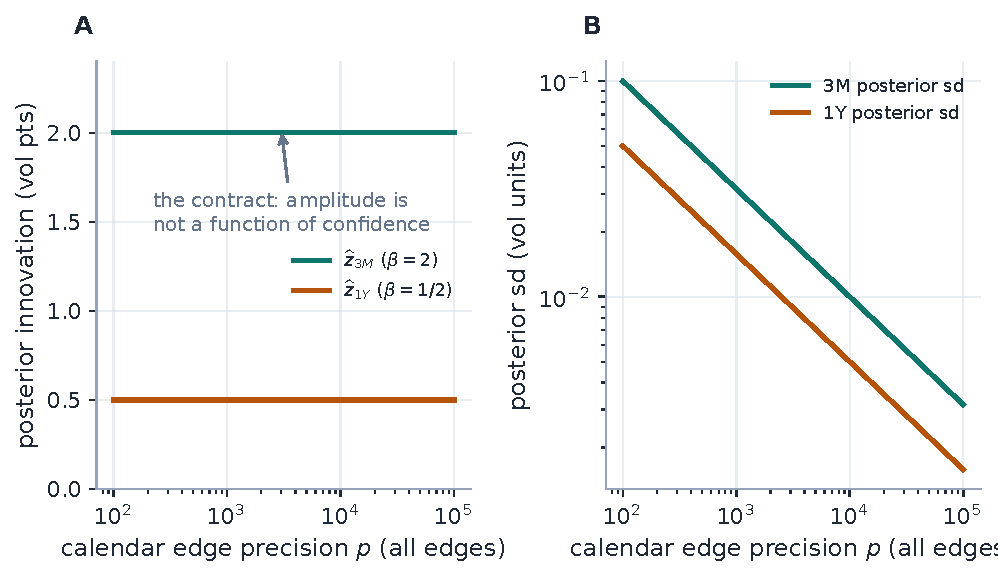
\includegraphics[width=\textwidth]{fig_gm_contract.pdf}
\caption{The contract, run through the production operator and posterior
(three-expiry ladder, 6M lit $+1$ vol point).  A: the dark receivers'
posterior means sit at the configured amplitudes $+2$ and $+0.5$
regardless of edge precision.  B: what the precision \emph{does} control
--- the posterior standard deviation, falling as $p^{-1/2}$.  Confidence
and amplitude are separate dials because they are separate fields of the
edge.}
\label{fig:contract}
\end{figure}

\subsection{Why pairwise factors: the operator that diluted its best
source}
\label{sec:rowform}

The specification's first draft boxed a different assembly: row-normalize
the incoming precisions, $K^p_{ij}=p_{ij}/q_i$, and charge each receiver
$q_i\,(z_i-\sum_jK^p_{ij}\beta_{ij}z_j)^2$.  Both forms produce the
identical receiver conditional of \cref{prop:conditional}, so every local
golden contract is blind to the choice.  They differ in the \emph{joint}
distribution, and the difference has teeth.

\begin{example}[title={Case file: the dead informer}]
\textbf{Setup.}  A receiver hears two informers at equal configured
precision: one lit, one \emph{dead} --- a dark dead-end with no lit path
and no other relations.

\textbf{Failure mode (row form).}  The averaging weights are fixed by
\emph{configured} precision even when an informer carries no information:
the row residual can be zeroed for any $z_i$ by moving the free informer,
so the posterior is improper, and under a small regularizing anchor the
receiver transfers only \gmdeadhalf\ of the lit message at equal
precisions --- decaying toward zero as the dead informer's configured
precision grows (\cref{fig:accountant}A).  Configuring trust in a silent
neighbour \emph{destroys} a live signal.

\textbf{The pairwise form.}  Marginalizing an unconstrained informer
removes its factor exactly --- the Gaussian integral over a free $z_j$ of
$p\,(z_i-\beta z_j)^2$ is flat in $z_i$ --- so the lit message passes at
full amplitude (production: transfer \gmpairflat\ across four decades of
dead-informer precision), the dead node simply rides along with a broad
marginal, and no improper direction survives the component solve.

\textbf{Two more reasons, one convention.}  A bidirectional reciprocal
pair collapses to \emph{one} factor, so auto-generated calendar relations
cannot double-count precision; and the factor list \emph{is} the sparse
assembly.  The convention that makes one-factor-per-relation well defined
is the canonical orientation: $p\,(z_i-\beta z_j)^2$ and
$p'\,(z_j-z_i/\beta)^2$ are the same factor iff
$p_{\mathrm{rev}}=p_{\mathrm{fwd}}/\beta^2$, so auto calendar relations
are quoted with the \emph{shorter} maturity as receiver (relation noise in
short-dated vol units, where desk intuition lives), the implied reverse
amplitude is $1/\beta$, and the receiver diagnostic $q_i$ maps every
incident factor into $i$'s units by that identity.  Explicit user edges
stay directed as entered --- entering both directions deliberately creates
two relations, and the cycle diagnostics of \cref{sec:diagnostics} apply.
\emph{The joint form of an operator is a modelling decision even when
every local conditional agrees.}
\end{example}

%======================================================================
\section{Amplitude: shape locked, level measured}
\label{sec:amplitude}

\subsection{The maturity shape}

For a calendar relation the amplitude is the locked maturity shape
\begin{equation}
\beta_{i\leftarrow j}=\Big(\frac{T_j}{T_i}\Big)^{\alpha_T},
\qquad \alpha_T=1\ \text{(default, per-handle configurable)}.
\label{eq:beta}
\end{equation}
$\alpha_T=1$ is constant total-variance injection --- a $+1$ vol-point
move at 6M reads as $+2$ at 3M and $+0.5$ at 1Y (\cref{fig:contract}) ---
and reciprocal by construction:
$\beta_{i\leftarrow j}\beta_{j\leftarrow i}=1$, so a calendar ladder
cannot claim amplification both ways.  The exponent is per-handle (ATM
level, skew and curvature need not share a maturity scaling; all default
$1$), and the Phase-0 study found the shape \emph{weakly identified} at
the day horizon ($R^2$ \gmshaperzero\ vs \gmshaperone\ across
$\alpha_T\in\{0,1\}$ once the level refits) --- so $1.0$ is retained for
its semantics, and the adjudication campaign sweeps it.

\subsection{The level is an empirical quantity}

Full-force transmission ($\widehat z=\beta z$ exactly) is the correct
semantics \emph{conditional on a relation the desk asserts}.  It is not
what the tape does on average: on $\sim$\gmcalpairs\ stored adjacent-pair
observations the realized day-over-day calendar transfer under the
$\alpha_T=1$ shape is \gmcallevel\ per unit of predicted move, and the
one-source index$\to$name transfer is \gmrhoindex.  A default that
transmits at full force would fail the pre-registered RMS gate on its
first day.  So amplitude splits: the \emph{shape} stays locked, and the
\emph{level} is a per-relation-class multiplier $\rho\in(0,1]$ with two
presets --- \texttt{desk} ($\rho=1$, full force, the belief mode) and
\texttt{learned} (the measured levels above; note they are
shape-dependent --- $0.34$ was the $\sqrt T$-shape calendar multiplier,
$0.23$ is the $\alpha_T=1$ value).

\subsection{The two wrong mechanizations, and the right one}

How should $\rho$ enter?  Two natural answers are provably wrong.
Scaling the beta ($\beta\to\rho\beta$) shrinks the forward conditional
but \emph{amplifies} the reverse one by $1/\rho$ --- the reciprocal
identity turns attenuation into amplification.  Emitting two directed
shrunk factors double-counts the relation and composes to
$2\rho/(1+\rho^2)\neq\rho$.  The mathematically consistent mechanization
of regression attenuation in both directions of one joint Gaussian is a
\emph{local innovation anchor}:
\begin{equation}
\kappa_i=p_{\mathrm{primary}}\,\frac{1-\rho_{\mathrm{class}}}
{\rho_{\mathrm{class}}},
\label{eq:anchor}
\end{equation}
with $p_{\mathrm{primary}}$ the largest incident relation precision in
node $i$'s units and $\rho_{\mathrm{class}}$ that primary relation's
class multiplier --- \emph{fixed at build time, never rescaled as further
edges arrive}.  The desk preset $\rho=1$ gives $\kappa=0$ exactly,
recovering the unamended contracts above.

\begin{proposition}[Corroboration under the node-linked anchor]
\label{prop:corroboration}
With $k$ equal agreeing clamped sources at precision $p$, beta one, and
the fixed anchor \eqref{eq:anchor}, the receiver's transfer per unit
message is
\[
\frac{kp}{\kappa+kp}=\frac{k\rho}{1-\rho+k\rho}:
\]
one source transfers exactly $\rho$; two lift it to $2\rho/(1+\rho)$;
independent corroboration keeps raising the effective transfer toward
one.
\end{proposition}

\begin{proof}
By \cref{prop:conditional} the $k$ agreeing messages average to the
common value at conditional precision $kp$; the anchor adds a
zero-innovation pseudo-message at precision $\kappa$, so the posterior
mean shrinks by $kp/(\kappa+kp)$; substitute \eqref{eq:anchor}.
\end{proof}

This is where the redesign earns the word \emph{measured}.  The competing
mechanization --- an edge-linked anchor
$\kappa_i=\sum_jp_{ij}(1-\rho)/\rho$, under which the transfer is
constant at $\rho$ regardless of source count --- makes a different
falsifiable prediction, and the stored benchmark rows adjudicate:
across \gmphasen\ name-days carrying same-sector peers, the one-source
index transfer slope is \gmrhoindex\ and the measured two-source
(index $+$ peer-average) slope is \gmtwosource\ --- a corroboration
uplift of $+\gmuplift\%$ against a pre-registered $\gmupliftbar\%$ bar.
Calibrating the fixed-$\kappa$ model on the \emph{single-source slope
alone} predicts \gmpredtwo\ for two sources: agreement to \gmpredgap\%,
with zero free parameters (\cref{fig:amplitude}).  The node-linked anchor
is not a preference; it is the mechanization the data chose.

\begin{figure}[H]
\centering
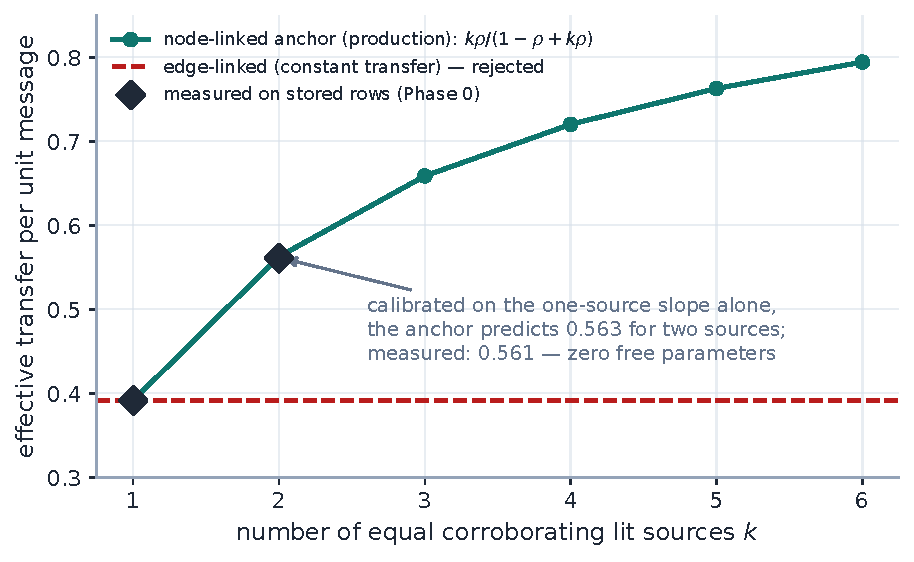
\includegraphics[width=0.9\textwidth]{fig_gm_amplitude.pdf}
\caption{Amplitude level as a measured object (production anchor and
posterior; measured points from the stored Phase-0 study artifact).  The
node-linked fixed anchor produces the corroboration curve
$k\rho/(1-\rho+k\rho)$; calibrated only on the one-source slope
(\gmrhoindex), it predicts the measured two-source transfer to
\gmpredgap\% with no free parameters.  The edge-linked alternative ---
constant transfer regardless of source count (dashed) --- is rejected by
the same measurement ($+\gmuplift\%$ uplift against a $\gmupliftbar\%$
bar).}
\label{fig:amplitude}
\end{figure}

\paragraph{Exercise 1.}
Derive both rejections of \cref{sec:amplitude}: (i) show that replacing
$\beta$ by $\rho\beta$ in one factor turns the implied reverse-direction
amplitude into $1/(\rho\beta)$; (ii) show that two directed factors
$p(z_i-\rho\beta z_j)^2+p'(z_j-\rho z_i/\beta)^2$ with matched units
produce a one-source transfer of $2\rho/(1+\rho^2)$, not $\rho$.  Then
verify from \eqref{eq:anchor} that $\rho=1$ gives $\kappa=0$ exactly ---
the desk preset is the contract semantics, not a limit.

%======================================================================
\section{Confidence: the precision families}
\label{sec:precision}

Amplitude answers ``how large''; precision answers ``how reliable'', and
the defaults are empirical.  The calendar family is
\begin{equation}
p^{\mathrm{cal}}_{ij}
=\frac{p_0}{\epsilon_T+\sqrt{|T_i-T_j|}},
\qquad
p_0\approx\gmpzero\ \text{vol}^{-2},\quad
\epsilon_T\approx\gmepst\ \sqrt{\text{years}},
\label{eq:calprec}
\end{equation}
with the seeds fitted on the same \gmcalpairs\ stored adjacent-pair
residuals (\cref{fig:calendar}B): about \gmtauonem\ vol points of
relation noise at a one-month gap, and --- the honest surprise ---
\emph{nearly gap-flat} at the day horizon: $\epsilon_T$ dominates, the
family degrades gracefully toward constant precision, and whether the
decay term earns its keep at all is one of the campaign's ablations
(\texttt{constant} and log-distance families ship beside it).  Cross-class
seeds from the same study: index$\to$name
$p\approx1.3\times10^4$, sector peer $p\approx0.9\times10^4$ (vol
units) --- with the recorded caveat that both are measured on ticker-day
\emph{median} innovations and are therefore upper bounds on per-edge
precision.

Two unit disciplines complete the picture.  \textbf{Per-handle units}:
edge precision is quoted in ATM-vol units; the skew and curvature fields
scale it by $(s_\sigma/s_h)^2$ with the production per-handle move scales
$(0.03,0.05,0.5)$ --- a units choice, not a semantics choice, since the
precision-weighted \emph{average} is invariant to a global rescale of all
incoming precisions.  \textbf{Variance is the readable coordinate}: an
edge carries $z_i=\beta z_j+\epsilon$, $\Var\,\epsilon=1/p$, so along a
chain amplitudes multiply while variances accumulate,
\begin{equation}
E[z_C]=\beta_2\beta_1\,E[z_A],
\qquad
\Var(z_C)=(\beta_2\beta_1)^2\Var(z_A)
+\frac{\beta_2^2}{p_1}+\frac{1}{p_2},
\label{eq:hops}
\end{equation}
and \emph{no mean haircut is ever applied for distance}
(\cref{fig:hops}): the mean crosses six hops undamped (production:
$\widehat z=\gmhopmean$ at hop six) while the band pays the toll, the
production marginals matching the accumulation identity to
\gmhopsdgap\ exactly.

\begin{figure}[H]
\centering
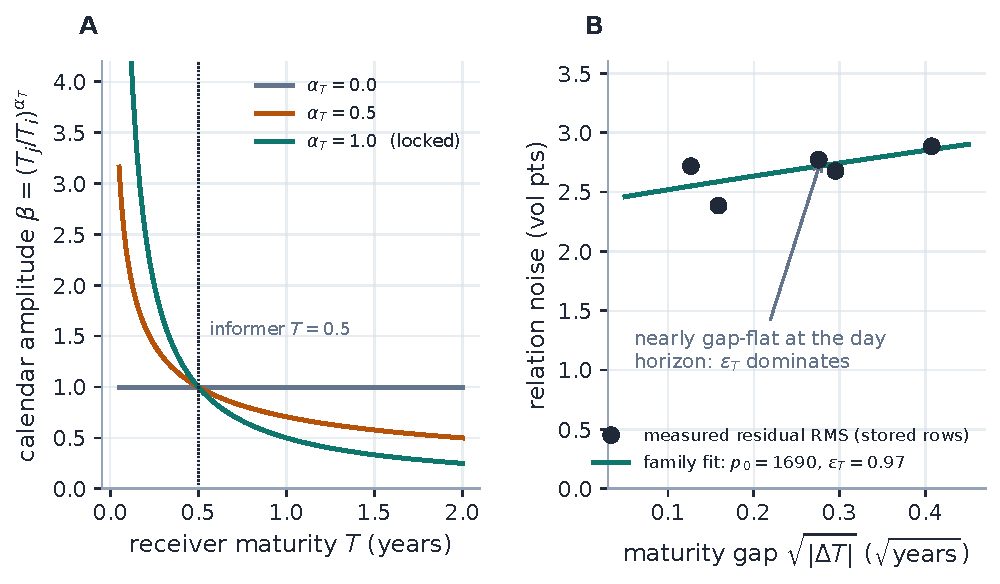
\includegraphics[width=\textwidth]{fig_gm_calendar.pdf}
\caption{The calendar relation, split into its two fields.  A: the
amplitude shape \eqref{eq:beta} --- what a 6M move implies elsewhere on
the ladder, per exponent; $\alpha_T=1$ (locked) is constant
total-variance injection.  B: the confidence family \eqref{eq:calprec}
against the stored residuals it was fitted on --- relation noise is
nearly gap-flat at the day horizon, so $\epsilon_T$ dominates and the
decay term's keep is an open ablation.}
\label{fig:calendar}
\end{figure}

\begin{figure}[H]
\centering
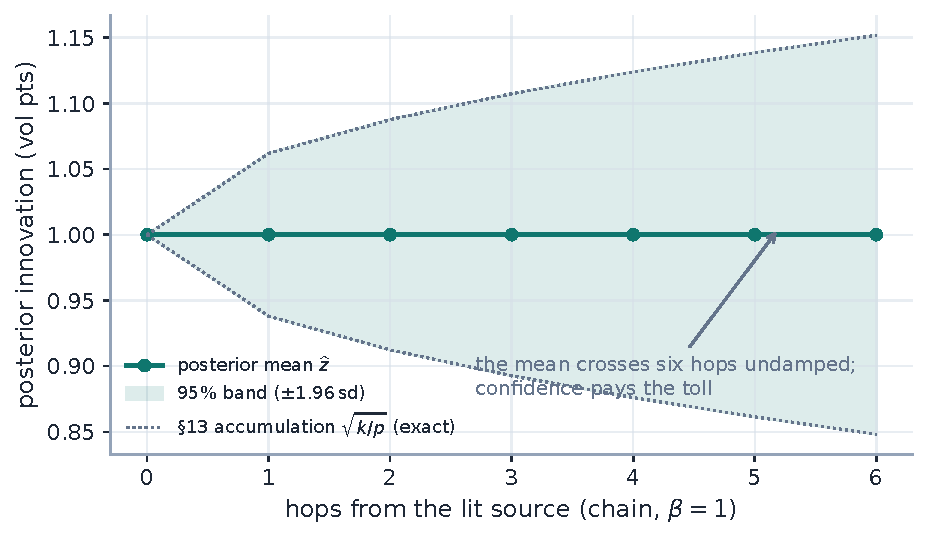
\includegraphics[width=0.88\textwidth]{fig_gm_hops.pdf}
\caption{Multi-hop propagation (production solve, six-hop chain,
$\beta=1$): the posterior mean crosses every hop undamped while the
marginal band accumulates exactly the per-edge relation variances of
\eqref{eq:hops} (dotted: the closed-form accumulation).  Distance costs
confidence, never amplitude --- the smooth field's coupled dial, uncoupled.}
\label{fig:hops}
\end{figure}

%======================================================================
\section{The accountant: the information-form posterior}
\label{sec:posterior}

The factors, the anchors and the lit observations assemble in information
form, solved per connected component of the factor support:
\begin{equation}
\boxed{\;
Q^+=\Qmsg+D_\kappa+H\T R_d H,
\qquad
b^+=H\T R_d\,d,
\qquad
\widehat z=(Q^+)^{-1}b^+,\quad \Sigma^+=(Q^+)^{-1},
\;}
\label{eq:posterior}
\end{equation}
with three honesty rules that are as load-bearing as the algebra.

\textbf{No lit path, no invented signal.}  Components are built on
$\beta\neq0$ edges (a zero-beta factor couples only its receiver --- the
reachability guard that stops an information-free informer from
destabilizing an observed component); a component with no lit observation
is never solved into propriety --- it keeps $\widehat z=0$, the
transported prior, a \texttt{no\_lit\_path} flag, and an explicitly broad
variance (one typical handle magnitude at the production layer).  Every
observed component is verified positive definite by Cholesky before
inversion.

\textbf{Innovations are only as precise as their ingredients.}  A lit
innovation is a difference of two estimates, so its observation precision
combines harmonically,
\begin{equation}
r^d_s=\Big(\frac{1}{r^{\mathrm{cal}}_s}+\frac{1}{p^0_s}\Big)^{-1},
\label{eq:rd}
\end{equation}
and the \emph{placement rule} holds baseline uncertainty to exactly one
appearance per node: folded into $r^d_s$ for a lit source, added once to
the reconstruction band for a dark node --- golden-locked so no node is
widened twice.

\textbf{Attribution is exact.}  The gain matrix $G=\Sigma^+H\T R_d$
decomposes every posterior shift over the observed lit sources,
$\widehat z_i=\sum_sG_{is}d_s$, contributions summing to the shift by
construction --- per independent \emph{source}, never per path, because
path contributions are correlated and non-unique.

The accountant's signature behaviours run through the production solve in
\cref{fig:accountant,fig:compete}.  Two routes carrying one source are
priced jointly: on the triangle fixture (source observed at finite
precision $p$, one direct and one two-leg route) the global posterior
variance is $\gmrepeatvar/p$ where naive per-message accounting --- the
\cref{eq:hops} effective precisions added as if independent --- claims
$\gmnaivevar/p$, overstating precision by $39\%$.  Competing messages
vote: equal opposing signals cancel to $\gmcompetecancel$ at
\emph{doubled} conditional precision $2p$ (disagreement is not silence);
a $3p$ source outvotes to $\gmcompeteout$; and under $\alpha_T=1$ betas
the same $\mp1$ raw signals land at $+\gmcompetebeta$ --- not a defect
but the contract: signals are mapped into receiver units \emph{before}
the vote, and equal-absolute-vol cancellation is a $\beta=1$ statement.

\begin{figure}[H]
\centering
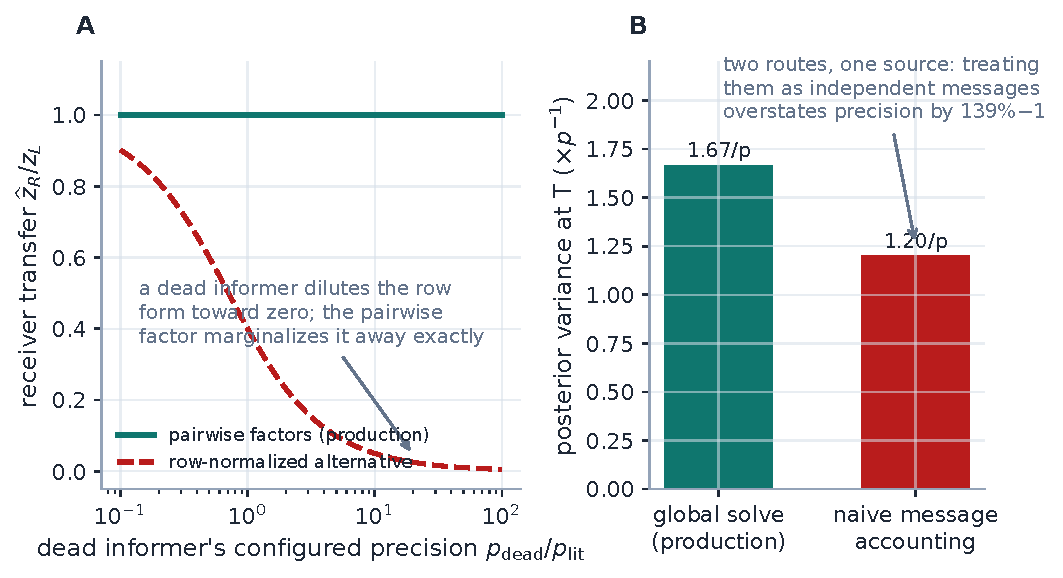
\includegraphics[width=\textwidth]{fig_gm_accountant.pdf}
\caption{The accountant at work (production solves).  A: the dead-informer
case file --- the rejected row-normalized operator dilutes a lit message
toward zero as a silent neighbour's \emph{configured} precision grows; the
pairwise factor marginalizes the dead informer away exactly.  B: repeated
routes from one source --- the global posterior variance
($\gmrepeatvar/p$) against naive independent-message accounting
($\gmnaivevar/p$): path counting would fabricate a $39\%$ precision
overstatement.}
\label{fig:accountant}
\end{figure}

\begin{figure}[H]
\centering
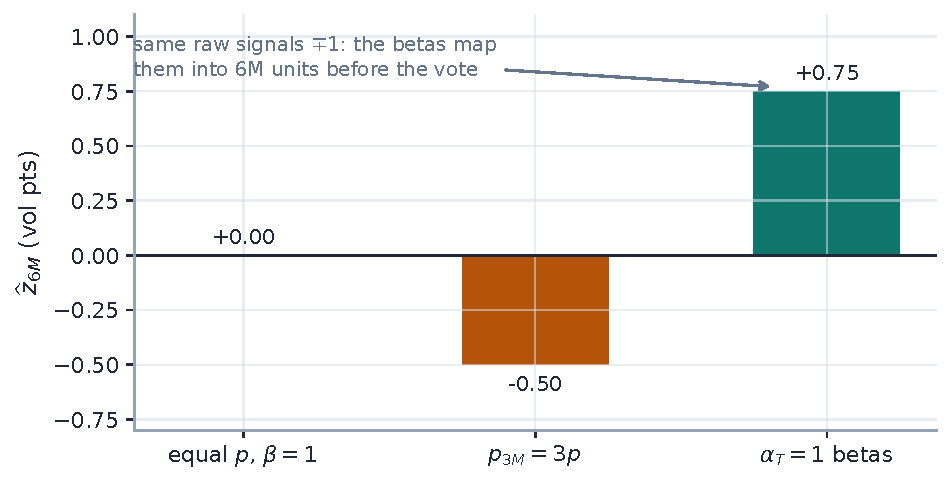
\includegraphics[width=0.88\textwidth]{fig_gm_compete.pdf}
\caption{Competing messages vote (production solves; 6M dark, 3M and 1Y
lit at $\mp1$ vol point).  Equal precision and $\beta=1$: exact
cancellation at doubled conditional precision.  A $3p$ source outvotes.
Under the locked $\alpha_T=1$ betas the same raw signals map to $-0.5$
and $+2$ in 6M units before averaging --- the receiver hears
receiver-unit predictions, not raw levels.}
\label{fig:compete}
\end{figure}

\paragraph{Exercise 2.}
Reproduce panel B of \cref{fig:accountant} by hand: with the source
observed at precision $p$ and all three relation precisions $p$, assemble
the $3\times3$ information matrix of \eqref{eq:posterior}, invert, and
show the target's marginal variance is exactly $5/(3p)$, while the
\cref{eq:hops} effective-message precisions ($p/2$ direct, $p/3$ through
the middle node) sum to $5p/6$, i.e.\ variance $6/(5p)$.  The naive
answer is wrong because both routes share the source's own uncertainty
--- the covariance the global solve refuses to forget.

\paragraph{Exercise 3.}
Three distinct quantities appear at every receiver: edge precision
$p_{ij}$, conditional incoming precision $q_i=\sum_jp_{ij}$, and marginal
posterior precision $1/\Sigma^+_{ii}$.  Construct a two-node example
where $q_i$ is large but the marginal precision is small (an uncertain
informer), and one where the marginal exceeds $q_i$ (the receiver's own
observation).  Only in the idealized clamped-independent-informer case do
the last two coincide --- which is why the wire reports both, and the UI
must never present $q_i$ as the final confidence.

%======================================================================
\section{Diagnostics and the gauge}
\label{sec:diagnostics}

Directedness in a Gaussian is a statement about the \emph{prediction
relation}, not about inference: the posterior precision is symmetric, so
observing a receiver legitimately updates an uncertain informer.  Where
strictly one-way conditioning is required, the graph must be a DAG or the
source clamped --- a UI arrow cannot create one-way Bayes.  What the
solver \emph{can} police is internal consistency of the amplitudes:

\begin{proposition}[Cycle consistency is a gauge condition]
\label{prop:gauge}
A positive beta structure is cycle-consistent --- every directed cycle's
beta product equals one --- iff there exist node potentials $g_i>0$ with
$\beta_{ij}=g_i/g_j$.
\end{proposition}

\begin{proof}
If $\beta_{ij}=g_i/g_j$, every cycle product telescopes to one.
Conversely, fix a spanning tree per component, set $\phi_i=\log g_i$ by
propagating $\log\beta$ along tree edges from an arbitrary root; a
non-tree edge with $\beta_{ij}\ne e^{\phi_i-\phi_j}$ closes a cycle whose
product is $\beta_{ij}e^{-(\phi_i-\phi_j)}\ne1$.
\end{proof}

Production runs exactly this proof as an algorithm: a union-find sweep
with logarithmic offsets assigns the potentials in linear time and flags
every closing edge whose implied cycle product strays from one (the
reference cross-check of \cref{app:ref} plants a consistent triangle ---
zero flags --- and an inconsistent one, flagged at product
\gmcyclebad).  Auto-generated calendar ladders are gauge-consistent by
construction ($g_i=T_i^{-\alpha_T}$); the diagnostic exists for explicit
edges, where an inconsistent loop means the configuration asserts
contradictory amplifications and the posterior will split the difference
somewhere the desk did not choose.  The wire also carries, per node, the
conditional $q_i$, the marginal precision, the \texttt{no\_lit\_path}
mask and the anchor provenance --- the three-quantity distinction of
Exercise~3 made permanently visible.

%======================================================================
\section{Production orchestration}
\label{sec:orchestration}

\subsection{Modes, and what feeds the solve}

\texttt{propagationMode} selects \texttt{smooth\_field} (the current
default --- byte-identical to the pre-revamp engine, locked by the full
legacy suite), \texttt{precision\_messages}, or \texttt{hybrid}
(message factors plus an explicit $\eta$-weighted legacy smoothness term;
config-only, and locked to coincide with pure message mode at $\eta=0$).
The message path reuses everything the legacy path computes --- selected
universe, transported priors and provenance tiers, lit innovations and
calibration precisions --- and feeds the same \texttt{HandleField} seam
back to reconstruction, functional bands, the idio floor, attribution and
the backtest, which run unchanged.  Auto relations over the selected
universe: one calendar factor per adjacent expiry pair per ticker
(canonical short receiver, \eqref{eq:calprec} precision) and one
beta-one cross factor per same-expiry ticker pair (constant precision,
orientation-neutral at beta one).  Persisted edge rules override auto;
request edges override both.  The observation-selection plan ports to the
information form through the $\Sigma^+$ columns --- the same rank-one
algebra, no covariance-form detour.

\subsection{Schema v2 and the direction migration}

The edge schema was rebuilt rather than overloaded:
\texttt{source/informer} $\to$ \texttt{target/receiver} naming, explicit
\texttt{messagePrecision}, three handle betas, relation class, and a
precision rule (\texttt{explicit} or \texttt{calendar\_distance}, the
latter re-deriving from \eqref{eq:calprec} on every solve).  The
migration confronted a recorded trap: the legacy engine's row convention
is $W[\mathrm{from}][\mathrm{to}]$ with \emph{``to'' informing ``from''}
--- the opposite of what parts of the schema documentation implied, hidden
for years by symmetric topologies.  The one-shot legacy import therefore
maps new receiver $=$ old \texttt{from} and new informer $=$ old
\texttt{to} --- the labels invert so the economics do not (test-locked)
--- and is explicit, never silent: legacy weight is a relative trust with
no canonical precision meaning, so the conversion factor is the caller's
stated choice and the legacy blob round-trips untouched.  The full edge
editor ships with the revamp: per-relation precision and betas, relation
class, inherited-versus-explicit display, implied-reverse chips,
seed-from-auto, receiver diagnostics, and a deterministic scenario
preview locked to the golden numbers of this note --- so a desk can
configure the three canonical examples and see these exact means before
saving.

\subsection{The six-node case file, revisited under message semantics}
\label{sec:sixnode}

The original note's miniature universe --- an SPX calendar chain, the
sector ETF XLK, two technology names --- reruns under the new operator
with the empirical seeds and \texttt{learned} amplitude presets
(\cref{fig:sixnode}; lit: SPX~3M $+1.00$ vol point, XLK~3M $+0.55$).
The table is generated by the production solve; the \texttt{desk} column
shows the same universe at $\rho=1$:

\begin{center}
\small
\begin{tabular}{llrrrr}
\toprule
Node & Role & $\widehat z$ (pts) & sd (pts) & desk $\widehat z$ & $q_i$\\
\midrule
\gmsixrows
\bottomrule
\end{tabular}
\end{center}

Every design choice is legible in the numbers.  SPX~1M inherits the index
move through the ladder at the $\alpha_T{=}1$ shape --- $+\gmsixspxmdesk$
points under desk force, shrunk to $+\gmsixspxm$ by the learned calendar
level, with the widest band in the universe (short-dated vol units are
where calendar noise is largest).  AAPL and MSFT each hear two
corroborating sources --- index and sector ETF --- so their transfer
($+\gmsixaapl$; desk $+\gmsixaapldesk$) sits \emph{above} what either
single-source level would give, exactly the corroboration lift of
\cref{prop:corroboration}.  And the conditional $q_i$ column differs from
the implied marginal everywhere --- the Exercise-3 distinction on
display.

\begin{figure}[H]
\centering
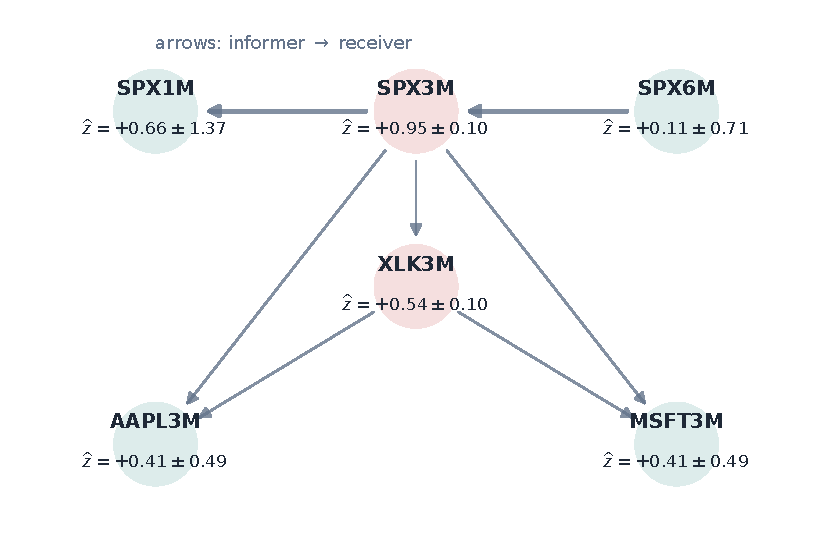
\includegraphics[width=0.9\textwidth]{fig_gm_sixnode.pdf}
\caption{The six-node case file under message semantics (production
solve; learned amplitude presets, Phase-0 precision seeds; arrows point
informer $\to$ receiver).  Lit nodes red, dark teal, each labelled with
its posterior innovation and marginal sd in vol points.  The names hear
index and ETF corroboration and transfer above the single-source level;
the 1M node shows the amplified-but-uncertain short end.}
\label{fig:sixnode}
\end{figure}

%======================================================================
\section{Evidence, recorded and in flight}
\label{sec:evidence}

\subsection{What the legacy engine already proved}

The smooth field's leave-one-out record is the floor any successor must
clear, and it stands: on the 25-asset, three-regime benchmark
($\sim$47k held-out scores, transport-regime bracketed), fully-dark
single names behind lit indexes and ETFs gain $+\gmspikeskilllo$ to
$+\gmspikeskillhi$ ATM vol bps in the August-2024 spike and
$+\gmhighskilllo$ to $+\gmhighskillhi$ fully out-of-sample in the
October-2022 bear, with calm-regime skill $+\gmcalmskilllo$ to
$+\gmcalmskillhi$ --- never negative --- and the once-dishonest calm
dark-name bands closed by the idiosyncratic ATM floor
($\operatorname{std}\zeta$ \gmidiobefore$\,\to\,$\gmidioafter\ and
\gmidiobeforetwo$\,\to\,$\gmidioaftertwo, mean-invariant by
construction).  Two recorded verdicts frame the revamp honestly.
\emph{The transient-name topology case file}: the harness once emitted
cross-asset edges one-way, making single names transient states of the
directed walk --- $\pi_i=0$, conductance zero, names disconnected, and a
measured ``$0.01$ bp response to a $96$ bp index move'' that was pure
artifact until the reverse-edge fix; the new operator's $q_i$ and
\texttt{no\_lit\_path} diagnostics would have named that failure on the
first run, which is itself an argument for contractual semantics.
\emph{The item-14 closure}: the learned-beta sweep met its liquid-split
activation rule but the gain was fractions of a bp (recorded, not
wired), and the OT term at $\lambda=1$ failed outright (negative skill,
$\zeta$ std blown to $1.3$--$2.6$) --- the smooth field's levers were
near their ceiling, which is why the redesign changes the operator rather
than the knobs.

\subsection{The Phase-0 design study and the smoke pair}

The redesign's own empirical base is the stored-row study already cited
throughout: transfer slopes \gmrhoindex\ (index) and \gmrhopeer\ (peer),
the corroboration adjudication of \cref{fig:amplitude}, the calendar
seeds of \cref{fig:calendar}, and the golden fixtures --- twenty-four
contracts locked against a brute-force Gaussian reference \emph{before}
the operator existed, then reproduced through it at $10^{-12}$.  One
single-pair smoke of the full production path is recorded with the
explicit caveat that one pair is not a verdict: message-learned full-LOO
ATM skill $+\gmsmokemsgfull/+\gmsmokemsgfullr$ bp against the legacy
$+\gmsmokelegfull/+\gmsmokelegfullr$, with the message bands slightly
narrow ($\zeta$ std \gmsmokemsgzeta) where the legacy's ran wide
(\gmsmokelegzeta).

\subsection{The pre-registered gate}
\label{sec:gate}

Precision messages become the product default \emph{only if}, on the
frozen three-regime fixtures over the strict out-of-sample window, the
combined campaign shows: material liquid-split dark-name skill over both
the transported prior and the current smooth field; no degradation in the
stressed regimes; no calm-regime harm beyond tolerance; $\zeta$ std near
one with 80/95\% band coverage near nominal after the idio floor; no
unstable cycles; and no wing-RMS deterioration.  Expectations were
recorded before the sweep: the \texttt{desk} preset is \emph{expected}
to lose day-horizon RMS (it is a belief mode and ships opt-in
regardless); the \texttt{learned} preset is the candidate; a
constant-precision ablation probes whether the gap-flat noise makes the
decay term superfluous.  The campaign --- six variants absorbing the
parked learned-betas sweep, band coverage added to the harness for the
occasion --- is running in the user's window as this note is built; its
parts land beside the frozen fixtures, and the decision table will be
filled from the artifact, not from enthusiasm.  Until then the default
stays \texttt{smooth\_field}, and everything in this note is reachable
one explicit mode switch away.

%======================================================================
\section{What is genuinely original here}
\label{sec:original}

Gaussian graphical models, information filters and gauge arguments are
classical; the synthesis is specific.  \emph{Contractual propagation for
volatility}: every desk-facing behaviour --- full-amplitude transfer,
precision addition, averaging, distance costing confidence not
amplitude --- is a golden test locked before implementation, so the
operator's semantics cannot drift.  \emph{Amplitude as shape times
measured level}, with the level mechanized through a node-linked anchor
whose corroboration law was validated on stored rows to \gmpredgap\%
with zero free parameters --- a design decision adjudicated by a
falsifiable prediction, not a preference.  \emph{The pairwise-factor
rejection of the row form} on dead-informer grounds
(\cref{fig:accountant}A): a joint-distribution defect invisible to every
local conditional, caught and documented before it shipped.
\emph{Honesty rules as first-class machinery}: no-lit-path components
left improper on purpose, baseline uncertainty placed exactly once,
attribution by source never by path.  And \emph{evidence discipline}:
the successor to a measurably skilful engine arrives with a
pre-registered gate and an in-flight adjudication rather than a default
flip.

%======================================================================
\section{Limitations}
\label{sec:limits}

Where the guarantees stop.  \emph{The adjudication is not in}: every
mean-semantics contract here is exact, but whether the message operator
\emph{predicts better} than the smooth field is precisely what the
running campaign decides, and this note refuses to pre-empt it ---
today's default remains the smooth field.  \emph{Correlated informers
overstate conditional precision}: $q_i$ adds configured precisions as if
sources were conditionally independent; the global solve prices shared
\emph{routes} correctly, but shared \emph{factors} (SPY and QQQ moving on
one macro shock) need class discounts or a common-factor node --- open,
with the marginal-vs-conditional gap on the wire as the tell.
\emph{Cross-class seeds are upper bounds} (ticker-median measurement);
per-edge noise will be higher.  \emph{The amplitude shape is weakly
identified at the day horizon} --- $\alpha_T=1$ is held by semantics, not
by $R^2$.  \emph{Hybrid mode is machinery, not a recommendation}
(validated only at its $\eta=0$ identity with pure messages).  \emph{The
solve is dense}, sized for the $O(10^2$--$10^3)$-node selected universe;
the factor list is sparse-ready and the sparse pass is deferred until a
universe demands it.  \emph{Calendar arbitrage remains soft}: calendar
factors propagate maturity signals but impose no hard cross-expiry
projection --- publish-time diagnostics and the LV projection remain the
fence.  And \emph{curvature stays the weakest handle} end to end, in
identification and in units, exactly as in the legacy engine.

\appendix
%======================================================================
\section{Hyperparameter atlas}
\label{app:atlas}

The only home for settings names: the body speaks mathematics, this
table speaks configuration.

\begingroup
\small
\begin{longtable}{p{0.32\textwidth}p{0.16\textwidth}p{0.44\textwidth}}
\caption{Message-mode hyperparameters (legacy smooth-field knobs are
unchanged and live in the original note's atlas).}\label{tab:atlas}\\
\toprule Knob & Default & Role\\ \midrule
\endfirsthead \toprule Knob & Default & Role\\ \midrule \endhead
\texttt{graphPropagationMode} & \texttt{smooth\_field} & The mode fork:
\texttt{smooth\_field} (byte-identical legacy) / \texttt{precision\_messages}
/ \texttt{hybrid} (config-only).\\
\texttt{calendarBetaExponent} & $1.0$ (per handle) & The amplitude shape
$\alpha_T$ of \eqref{eq:beta}.\\
\texttt{calendarAmplitude} & $1.0$ & Calendar level $\rho$; presets desk
$=1.0$ / learned $\approx0.23$ (the $\alpha_T{=}1$ value).\\
\texttt{crossAmplitude} & $1.0$ & Shared level $\rho$ for every cross
relation class in v1; learned $\approx0.39$ index.\\
\texttt{calendarPrecisionScale} $p_0$ & $1.7\times10^3$ & Calendar
precision scale \eqref{eq:calprec}, Phase-0 seed.\\
\texttt{calendarPrecisionEpsilon} $\epsilon_T$ & $0.97$ & Near-identical-
expiry precision cap; dominates at the day horizon.\\
\texttt{calendarPrecisionDecay} & \texttt{inverse\_sqrt\_gap} & Family:
inverse-sqrt-gap / constant / log-distance.\\
\texttt{crossPrecisionScale} & $1.3\times10^4$ & Constant cross-relation
precision (Phase-0 index seed; upper bound).\\
\texttt{innovationAnchorPrecision} & derived & Override for
\eqref{eq:anchor}; unset $=$ node-linked from $\rho$, and $\rho=1$ gives
$\kappa=0$ exactly.\\
\texttt{cycleBetaTolerance} & $10^{-9}$ & Gauge-sweep flag threshold
(\cref{prop:gauge}).\\
\texttt{messageEdges} / persisted rules & --- & Request edges $\to$
persisted schema-v2 rules $\to$ auto relations, in that precedence.\\
\midrule
\multicolumn{3}{l}{\emph{Hidden (module constants)}}\\ \midrule
\texttt{HANDLE\_PRECISION\_SCALE} & $(1,0.36,0.0036)$ & The
$(s_\sigma/s_h)^2$ per-handle precision units of \cref{sec:precision}.\\
\texttt{RELATION\_CLASSES} & 5 classes & calendar / broad\_index /
sector\_etf / sector\_peer / custom.\\
\texttt{DISCONNECTED\_Z\_SD} & $(0.03,0.05,0.5)$ & The honest
no-lit-path innovation sd per handle (one typical move).\\
canonical orientation & shorter $T$ & Auto calendar receiver; reverse
identity $p_{\mathrm{rev}}=p_{\mathrm{fwd}}/\beta^2$.\\
\bottomrule
\end{longtable}
\endgroup

%======================================================================
\section{Performance notes}
\label{app:perf}

\begin{enumerate}[leftmargin=1.6em]
\item \textbf{The assembly is the factor list}: $O(E)$ triplets, dense
materialization at the current $O(10^2$--$10^3)$-node design point, and
the existing 1k-node perf rail passes unchanged.  Sparse Cholesky /
selected-inverse marginals are the deferred scale pass --- the pairwise
form was chosen partly because it sparsifies without renormalization
coupling.
\item \textbf{Per-component solves}: the posterior inverts each factor-
support component separately, so one disconnected block never pays for
another, and the Cholesky PD guard localizes any conditioning failure to
a named component.
\item \textbf{The message path adds no new data work}: universe,
transported priors, innovations and calibration precisions are the same
objects the legacy path computes; the mode fork is downstream of all of
them.
\item \textbf{Adjudication runs where long jobs survive}: the campaign
executes from the user's own shell (chunked, resumable parts beside the
frozen fixtures); tool-spawned background jobs are killed on this box,
which is a recorded operational constraint, not a suggestion.
\item No benchmark in this note was re-timed; figures and macros were
generated at commit \texttt{\gmgencommit} on \gmgendate, golden numbers
through the production modules and empirical numbers from the stored
Phase-0 artifact.
\end{enumerate}

%======================================================================
\section{Traceability}
\label{app:trace}

\begingroup
\small
\setlength{\tabcolsep}{3pt}
\begin{longtable}{@{}p{0.33\textwidth}p{0.15\textwidth}p{0.24\textwidth}p{0.23\textwidth}@{}}
\caption{Claims in this note and the code/tests that lock them.}\\
\toprule Claim & Object & Code anchor & Test anchor\\ \midrule
\endfirsthead
\toprule Claim & Object & Code anchor & Test anchor\\ \midrule
\endhead
Pairwise operator PSD; receiver conditional; $q_i$ unit mapping;
canonical orientation &
\eqref{eq:qmsg}, \cref{prop:conditional} &
\nolinkurl{volfit/graph/message.py} &
\nolinkurl{test_graph_message.py}\\
Golden contracts locked before code (transmission, competition,
cross-asset, multi-hop, dead informer, repeated path, shrunk mode,
baseline-once) &
\cref{sec:contracts,sec:amplitude,sec:posterior} &
\nolinkurl{tests/fixtures/graph_message_golden.json} &
\nolinkurl{test_graph_message_golden.py} (brute-force reference),
\nolinkurl{test_graph_message.py}\\
Information-form component solve; no-lit honesty; reachability guard;
exact attribution &
\eqref{eq:posterior} &
\nolinkurl{volfit/graph/message_posterior.py} &
\nolinkurl{test_graph_message_posterior.py}\\
Node-linked anchor $\kappa=p(1-\rho)/\rho$ fixed at build;
$\rho=1\Rightarrow\kappa=0$; corroboration law &
\eqref{eq:anchor}, \cref{prop:corroboration} &
\nolinkurl{volfit/graph/message.py} &
\nolinkurl{test_graph_message.py},
\nolinkurl{test_graph_message_golden.py}\\
Cycle gauge sweep flags inconsistent products &
\cref{prop:gauge} &
\nolinkurl{volfit/graph/message.py} &
\nolinkurl{test_graph_message.py}\\
Production orchestration: auto relations, $r^d$ harmonic, band
placement, mode fork, hybrid $\equiv$ message at $\eta=0$ &
\cref{sec:orchestration} &
\nolinkurl{volfit/api/graph_message.py},
\nolinkurl{api/graph_extrapolation.py} &
\nolinkurl{test_graph_message_production.py}\\
Schema v2; legacy-import direction inversion preserves economics;
legacy blob untouched &
\cref{sec:orchestration} &
\nolinkurl{api/schemas.py} (\texttt{GraphMessageEdge}),
\nolinkurl{api/graph_message.py} &
\nolinkurl{test_graph_message_production.py}\\
Smooth-field byte identity at defaults &
invariant 6 &
\nolinkurl{volfit/graph/\{prior,posterior\}.py} &
legacy suite unmodified (1302 green),
\nolinkurl{test_graph_example.py}\\
Adjudication harness variants, coverage metrics, decision table &
\cref{sec:gate} &
\nolinkurl{backtest/run_message_adjudication.ps1},
\nolinkurl{backtest/graph_edges.py} &
\nolinkurl{test_message_adjudication.py}\\
Legacy 25-asset verdict; transient-name topology fix; idio floor &
\cref{sec:evidence} &
\nolinkurl{backtest/graph_loo.py},
\nolinkurl{volfit/graph/idio.py} &
\nolinkurl{test_graph_loo_backtest.py},
\nolinkurl{test_graph_idio.py}\\
Phase-0 study (anchor choice, seeds, learned levels) &
\cref{sec:amplitude,sec:precision} &
\nolinkurl{backtest/message_phase0.py} &
artifact \nolinkurl{results/message_phase0.json} (regenerable)\\
\bottomrule
\end{longtable}
\endgroup

%======================================================================
\section{Reference implementation}
\label{app:ref}

The operator and the posterior are each a few lines.  Executed against
the production modules on a four-node directed universe with a
node-linked anchor (operator matrix, posterior mean, marginal
variances), the maximum deviation is \gmrefagree; the gauge sweep
cross-check flags nothing on a consistent triangle
(\gmcycleflags\ flags) and reports the planted inconsistent product
\gmcyclebad\ on the broken one.

\begin{lstlisting}[caption={The pairwise operator and the information-form
solve (verified against \texttt{graph/message.py} and
\texttt{graph/message\_posterior.py}; agreement stated above).}]
def message_operator(n, factors):        # factors: (i, j, p, beta)
    Q = np.zeros((n, n))
    for i, j, p, b in factors:
        u = np.zeros(n); u[i] = 1.0; u[j] = -b
        Q += p * np.outer(u, u)          # PSD for any real beta
    return Q

def message_posterior(Q, kappa, obs, d, r):
    Qp = Q + np.diag(kappa)          # anchors (0 in desk mode)
    b = np.zeros(len(Q))
    Qp[obs, obs] += r                # H^T R H
    b[obs] += r * d                  # H^T R d
    Sigma = np.linalg.inv(Qp)        # per lit component
    return Sigma @ b, Sigma          # z_hat, covariance
\end{lstlisting}

\begin{thebibliography}{9}
\bibitem{RasmussenWilliams2006} C.~Rasmussen and C.~Williams.
\emph{Gaussian Processes for Machine Learning}. MIT Press, 2006.
\bibitem{Koller2009} D.~Koller and N.~Friedman. \emph{Probabilistic
Graphical Models}. MIT Press, 2009.
\bibitem{Pearl1988} J.~Pearl. \emph{Probabilistic Reasoning in
Intelligent Systems}. Morgan Kaufmann, 1988.
\bibitem{Peyre2019} G.~Peyr\'e and M.~Cuturi. Computational optimal
transport. \emph{Found.\ Trends Mach.\ Learn.}, 11(5--6):355--607, 2019.
\end{thebibliography}

\end{document}
